% ============================================================
%  يُترجَم بـ XeLaTeX  (في Overleaf: Menu → Compiler → XeLaTeX)
%  الخط: Amiri (متوفر في Overleaf، أو حمّله من github.com/aliftype/amiri)
% ============================================================
\documentclass[12pt,a4paper]{article}
\usepackage[a4paper,margin=1.2cm,top=2.3cm,bottom=2.9cm,headheight=15pt,footskip=1.5cm]{geometry}
\usepackage{amsmath,amssymb}
\usepackage{icomma}
\usepackage[english,bidi=default,layout=lists]{babel}
\babelprovide[import,main]{arabic}
\babelfont{rm}[Scale=1.08]{Amiri}
\babelfont{sf}[Scale=1.08]{Amiri}
\usepackage[most]{tcolorbox}
\usepackage{tikz}
\usetikzlibrary{arrows.meta,calc,shadings}
\usepackage{array}
\usepackage{colortbl}
\usepackage{fancyhdr}
\usepackage{titlesec}
\usepackage{enumitem}
\usepackage{collcell}
\usepackage{needspace}
\usepackage{etoolbox}
\newcolumntype{C}{>{\collectcell\ar}c<{\endcollectcell}}
\pretocmd{\section}{\Needspace{15\baselineskip}}{}{}
\pretocmd{\subsection}{\Needspace{11\baselineskip}}{}{}

\definecolor{cDef}{HTML}{1F4E9C}
\definecolor{cThm}{HTML}{B3261E}
\definecolor{cRem}{HTML}{2E7D32}
\definecolor{cEx}{HTML}{C76B00}
\definecolor{cMeth}{HTML}{6A1B9A}
\definecolor{cSol}{HTML}{00695C}
\definecolor{cSec}{HTML}{1F3A68}

\titleformat{\section}{\Large\bfseries\color{cSec}}{\thesection.}{0.6em}{}[{\color{cSec!60}\titlerule[1pt]}]
\titleformat{\subsection}{\large\bfseries\color{cThm!85!black}}{\thesubsection.}{0.5em}{}
\titlespacing*{\section}{0pt}{14pt}{8pt}
\titlespacing*{\subsection}{0pt}{10pt}{5pt}
\setlength{\parindent}{0pt}
\setlength{\parskip}{4pt}
\setlist{itemsep=2pt,topsep=3pt}

\newtcolorbox{arbox}[3][]{enhanced,
  colback=#2!5,colframe=#2!80!black,arc=2mm,boxrule=0.8pt,
  left=6pt,right=6pt,top=8pt,bottom=5pt,
  fonttitle=\bfseries,coltitle=white,
  title={\foreignlanguage{arabic}{#3}},
  attach boxed title to top right={xshift=-5mm,yshift=-3mm},
  boxed title style={colback=#2!80!black,arc=1.5mm,boxrule=0pt},
  before upper={\selectlanguage{arabic}},
  before skip=8pt,after skip=8pt,breakable,#1}
\newenvironment{BOX}[2]{\begin{otherlanguage}{english}\begin{arbox}{#1}{#2}}{\end{arbox}\end{otherlanguage}}
\newenvironment{tarif}[1][تعريف]{\begin{BOX}{cDef}{#1}}{\end{BOX}}
\newenvironment{khassia}[1][خاصية]{\begin{BOX}{cThm}{#1}}{\end{BOX}}
\newenvironment{molahada}[1][ملاحظة]{\begin{BOX}{cRem}{#1}}{\end{BOX}}
\newenvironment{mithal}[1][مثال]{\begin{BOX}{cEx}{#1}}{\end{BOX}}
\newenvironment{tariqa}[1][طريقة]{\begin{BOX}{cMeth}{#1}}{\end{BOX}}

\newcounter{exo}
\newenvironment{tamrin}[1]{\stepcounter{exo}\begin{BOX}{cSec}{التمرين \theexo: #1}}{\end{BOX}}
\newenvironment{hal}{\Needspace{12\baselineskip}\begin{otherlanguage}{english}\begin{arbox}[breakable]{cSol}{حل التمرين \theexo}}{\end{arbox}\end{otherlanguage}}

\newenvironment{LTR}{\begin{otherlanguage}{english}}{\end{otherlanguage}}
\newcommand{\ar}[1]{\foreignlanguage{arabic}{#1}}

\renewcommand{\dots}{\mathinner{\ldotp\ldotp\ldotp}}
\renewcommand{\ldots}{\mathinner{\ldotp\ldotp\ldotp}}
\renewcommand{\cdots}{\mathinner{\cdotp\cdotp\cdotp}}
\newcommand{\N}{\mathbb{N}}
\newcommand{\Z}{\mathbb{Z}}
\newcommand{\D}{\mathbb{D}}
\newcommand{\Q}{\mathbb{Q}}
\newcommand{\R}{\mathbb{R}}
\newcommand{\pgcd}{\operatorname{PGCD}}
\newcommand{\ppcm}{\operatorname{PPCM}}

% \NLseg{a}{b}{[}{]} ; \NLright{a}{[} ; \NLleft{b}{]}  (interval on a number line)
\newcommand{\NLseg}[4]{\begin{LTR}\begin{tikzpicture}[baseline=-0.6ex]
 \draw[-{Stealth[length=2mm]},gray!70](0,0)--(3.4,0);
 \draw[line width=2pt,cThm!80!black](0.7,0)--(2.7,0);
 \node[cThm!80!black,font=\LARGE] at (0.7,0){$#3$};
 \node[cThm!80!black,font=\LARGE] at (2.7,0){$#4$};
 \node[below=3pt,font=\footnotesize] at (0.7,0){$#1$};
 \node[below=3pt,font=\footnotesize] at (2.7,0){$#2$};
\end{tikzpicture}\end{LTR}}
\newcommand{\NLright}[2]{\begin{LTR}\begin{tikzpicture}[baseline=-0.6ex]
 \draw[-{Stealth[length=2mm]},gray!70](0,0)--(3.4,0);
 \draw[line width=2pt,cThm!80!black](1.3,0)--(3.3,0);
 \node[cThm!80!black,font=\LARGE] at (1.3,0){$#2$};
 \node[below=3pt,font=\footnotesize] at (1.3,0){$#1$};
\end{tikzpicture}\end{LTR}}
\newcommand{\NLleft}[2]{\begin{LTR}\begin{tikzpicture}[baseline=-0.6ex]
 \draw[-{Stealth[length=2mm]},gray!70](0,0)--(3.4,0);
 \draw[line width=2pt,cThm!80!black](0.05,0)--(2.1,0);
 \node[cThm!80!black,font=\LARGE] at (2.1,0){$#2$};
 \node[below=3pt,font=\footnotesize] at (2.1,0){$#1$};
\end{tikzpicture}\end{LTR}}

% ---------- social-media icons (pure TikZ) ----------
\definecolor{cFB}{HTML}{1877F2}
\definecolor{cTG}{HTML}{229ED9}
\definecolor{cIG1}{HTML}{FEDA75}
\definecolor{cIG2}{HTML}{D62976}
\definecolor{cIG3}{HTML}{4F5BD5}
\newcommand{\fbicon}{\begin{LTR}\begin{tikzpicture}[baseline=-0.75ex,x=1em,y=1em]
 \fill[cFB] (0,0) circle (0.55);
 \node[white,inner sep=0,font=\usefont{TU}{lmss}{bx}{n}\small] at (0.04,-0.02) {f};
\end{tikzpicture}\end{LTR}}
\newcommand{\igicon}{\begin{LTR}
\begin{tikzpicture}[baseline=-0.75ex,x=1em,y=1em]
 \shade[lower left=cIG1,lower right=cIG2,upper left=cIG2,upper right=cIG3,rounded corners=0.28em] (-0.55,-0.55) rectangle (0.55,0.55);
 \draw[white,line width=0.09em,rounded corners=0.18em] (-0.36,-0.36) rectangle (0.36,0.36);
 \draw[white,line width=0.09em] (0,0) circle (0.17);
 \fill[white] (0.22,0.22) circle (0.05);
\end{tikzpicture}\end{LTR}}
\newcommand{\tgicon}{\begin{LTR}
\begin{tikzpicture}[baseline=-0.75ex,x=1em,y=1em]
 \fill[cTG] (0,0) circle (0.55);
 \fill[white] (-0.33,0.0) -- (0.32,0.27) -- (0.2,-0.3) -- (0.0,-0.15) -- (-0.08,-0.28) -- (-0.08,-0.08) -- cycle;
 \fill[cTG!70!black] (-0.08,-0.08) -- (0.25,0.2) -- (0.0,-0.15) -- (-0.08,-0.28) -- cycle;
\end{tikzpicture}\end{LTR}}
% page number: black box, white two-digit number, at the right of the social row
\newcommand{\PageBox}{\begin{LTR}\tikz[baseline=(p.base)]\node[fill=black,text=white,inner sep=2.5pt,minimum width=1.6em,minimum height=1.3em,font=\usefont{TU}{lmss}{bx}{n}\small](p){\ifnum\value{page}<10 0\fi\arabic{page}};\end{LTR}}
% visual left-to-right order: Telegram | Instagram | Facebook | page box
\newcommand{\SocialRow}{\begin{otherlanguage}{english}%
 \ar{\textbf{الأستاذ سوايسية هشام للرياضيات}}\ \tgicon\hfill
 \textbf{prof\_hicham\_math}\ \igicon\hfill
 \ar{\textbf{الأستاذ سوايسية هشام للرياضيات}}\ \fbicon\hspace{2.2em}\PageBox\end{otherlanguage}}

\pagestyle{fancy}
\fancyhf{}
\renewcommand{\headrulewidth}{0.6pt}
\renewcommand{\footrulewidth}{0.4pt}
% \SetHeader{right head: document title}{left head: level -- stream}
\newcommand{\SetHeader}[2]{%
 \fancyhead[C]{\parbox{\textwidth}{\ar{#1\hfill #2}}}%
 \fancyfoot[C]{\parbox{\textwidth}{\small\SocialRow}}}
\usepackage{tkz-tab}
\usepackage{multicol}
% variation / sign table (LTR)
\newenvironment{TAB}{\par\begin{center}\begin{LTR}\begin{tikzpicture}[scale=0.95,every node/.style={font=\small}]}{\end{tikzpicture}\end{LTR}\end{center}}
% grid + axes, clipped: \begin{GR}{xmin}{xmax}{ymin}{ymax}{unit cm}
\newenvironment{GR}[5]{\par\begin{center}\begin{LTR}\begin{tikzpicture}[x=#5cm,y=#5cm,font=\footnotesize]
 \draw[gray!25,very thin] (#1,#3) grid (#2,#4);
 \draw[-{Stealth[length=2mm]}] (#1,0)--(#2+0.3,0) node[below left]{$x$};
 \draw[-{Stealth[length=2mm]}] (0,#3)--(0,#4+0.3) node[below left]{$y$};
 \node[below left] at (0,0){$O$};
 \begin{scope}\clip (#1,#3) rectangle (#2,#4);}
{\end{scope}\end{tikzpicture}\end{LTR}\end{center}}
\newcommand{\Ticks}[2]{\foreach \t in {#1} \node[below,font=\scriptsize] at (\t,0){$\t$}; \foreach \t in {#2} \node[left,font=\scriptsize] at (0,\t){$\t$};}
\newcommand{\bx}[1]{\ensuremath{\colorbox{cDef!12}{$\displaystyle #1$}}}
\newcommand{\TwoCol}[4]{\par\begin{LTR}\noindent\begin{minipage}[t]{#1\textwidth}\selectlanguage{arabic}#2\end{minipage}\hfill\begin{minipage}[t]{#3\textwidth}\selectlanguage{arabic}#4\end{minipage}\end{LTR}\par}
\newcommand{\RL}[4]{\TwoCol{#3}{#4}{#1}{#2}}  % \RL{w1}{right content}{w2}{left content}
\newcommand{\ok}{$\textcolor{cRem}{\checkmark}$}
\newcommand{\limn}{\displaystyle\lim_{n\to+\infty}}
% sub-questions, each on its own line
\newenvironment{sq}{\begin{itemize}[leftmargin=2.4em,itemsep=3pt]}{\end{itemize}}
\newcommand{\qa}{\item[(أ)]}\newcommand{\qb}{\item[(ب)]}\newcommand{\qc}{\item[(جـ)]}\newcommand{\qd}{\item[(د)]}\newcommand{\qe}{\item[(هـ)]}
\newcommand{\pa}{\par\smallskip\textbf{(أ)} }\newcommand{\pb}{\par\smallskip\textbf{(ب)} }\newcommand{\pc}{\par\smallskip\textbf{(جـ)} }\newcommand{\pd}{\par\smallskip\textbf{(د)} }\newcommand{\pe}{\par\smallskip\textbf{(هـ)} }
\newcommand{\QQ}[1]{\par\smallskip\textbf{#1.} }
\newenvironment{tmr}{\stepcounter{exo}\begin{BOX}{cSec}{تمرين محلول \theexo}}{\end{BOX}}
\newcommand{\ABC}[3]{\\[2pt]\begin{tabular}{p{0.28\textwidth}p{0.28\textwidth}p{0.28\textwidth}}(جـ) \ #3 & (ب) \ #2 & (أ) \ #1\end{tabular}}
\pretocmd{\section}{\Needspace{24\baselineskip}}{}{}
\newtcbox{\bxtbox}{on line,colback=cDef!12,colframe=cDef!12,boxrule=0pt,arc=1pt,boxsep=0pt,left=2pt,right=2pt,top=1pt,bottom=1pt}
\newcommand{\bxt}[1]{\foreignlanguage{english}{\bxtbox{\ar{#1}}}}
\usepackage{longtable}
\setlength{\LTpre}{4pt}\setlength{\LTpost}{0pt}
\newcommand{\Phase}[1]{\textbf{#1}}
\newcommand{\Fld}[2]{\textbf{#1:}\ #2}
% رأس المذكرة على نمط النموذج: إطار بعنوان «مذكرة رقم»، معلومات الحصة، ثم إطار الكفاءات
\newcommand{\ModhHead}[9]{%
\begin{LTR}
\begin{tcolorbox}[enhanced,colback=white,colframe=cThm!85!black,arc=4mm,boxrule=1pt,top=14pt,bottom=6pt,left=8pt,right=8pt,
 overlay={\node[fill=cThm!85!black,text=white,rounded corners=3mm,inner xsep=14pt,inner ysep=4pt,font=\large\bfseries] at ([yshift=0pt]frame.north){\ar{مذكرة رقم #1}};},
 before upper={\selectlanguage{arabic}}]
\begin{tabular}{@{}p{0.4\linewidth}p{0.55\linewidth}@{}}
\Fld{المستوى}{#2} & \Fld{الثانوية}{\dotfill}\\[3pt]
\Fld{المادة}{رياضيات} & \Fld{ميدان التعلم}{#3}\\[3pt]
\Fld{المدة}{#5} & \Fld{الوحدة التعلمية}{#4}\\[3pt]
\Fld{الأستاذ}{\dotfill} & \Fld{المحتوى المعرفي}{#6}\\
\end{tabular}
\end{tcolorbox}
\begin{tcolorbox}[enhanced,colback=white,colframe=cThm!85!black,arc=3mm,boxrule=0.8pt,sidebyside,sidebyside align=top,lefthand ratio=0.5,
 segmentation style={dashed,cThm!60},before upper={\selectlanguage{arabic}},before lower={\selectlanguage{arabic}}]
\textbf{الكفاءات المستهدفة:}\par #8
\tcblower
\textbf{الكفاءات القبلية:}\par #7
\end{tcolorbox}
\end{LTR}
\par\smallskip\textbf{الوسائل:} #9\par\smallskip}
\newenvironment{Sayr}{%
\begin{LTR}\renewcommand{\arraystretch}{1.25}\setlength{\tabcolsep}{4pt}\relpenalty=10000\binoppenalty=10000\tolerance=9000\emergencystretch=0.3\linewidth
\begin{longtable}{|p{0.09\textwidth}|>{\centering\arraybackslash}p{0.05\textwidth}|p{0.71\textwidth}|>{\centering\arraybackslash}p{0.09\textwidth}|}
\hline\rowcolor{cThm!12}\ar{\footnotesize\textbf{توجيهات وتعاليق}} & \ar{\footnotesize\textbf{المدة}} & \ar{\textbf{سير الحصة}} & \ar{\footnotesize\textbf{مراحل الحصة}}\\\hline\endhead
\hline\endfoot}{\end{longtable}\end{LTR}}
% سطر في الجدول: \Row{مرحلة}{سير}{مدة}{توجيهات}
\newcommand{\RaggedEnd}{\leftskip=0pt plus 1fil\relax}
\newcommand{\Row}[4]{\ar{\small #4} & \ar{#3} & \ar{\RaggedEnd #2} & \cellcolor{cThm!8}\ar{\Phase{#1}}\\\hline}

\newcommand{\Lab}[2]{\foreignlanguage{english}{\tcbox[on line,colback=#1,colframe=#1,boxrule=0pt,arc=2pt,boxsep=1pt,left=5pt,right=5pt,top=1pt,bottom=1pt]{\ar{\textcolor{white}{\textbf{#2}}}}}}
\newcommand{\Num}[1]{\foreignlanguage{english}{\tikz[baseline=(c.base)]\node[fill=cDef,text=white,inner sep=2pt,font=\footnotesize\bfseries](c){#1};}}
\newcommand{\ck}{\ensuremath{{\color{cRem}\checkmark}}}
\newenvironment{Kad}[1]{\par\smallskip\Lab{#1}}{\par}
\newcommand{\RR}[1]{\ifmmode{\color{cThm}#1}\else$\mbox{\color{cThm}#1}$\fi}
\newcommand{\T}[1]{$\mbox{\color{cDef}\bfseries #1}$}
\SetHeader{\small\bfseries\color{cSec}مذكرات محور: الدالة الأسية}{\small\color{cSec}السنة الثالثة ثانوي -- علوم تجريبية}
\begin{document}
\begin{LTR}
\begin{tcolorbox}[enhanced,colback=cThm!85!black,colframe=cThm!85!black,arc=3mm,halign=center,boxrule=0pt,top=12pt,bottom=12pt,before upper={\selectlanguage{arabic}}]
{\color{white}\fontsize{24}{30}\selectfont\bfseries مذكرات محور: الدالة الأسية}\\[8pt]
{\color{white}\large السنة الثالثة ثانوي -- علوم تجريبية}\\[4pt]
{\color{white}\large 4 مذكرات (8 ساعات) -- السنة الدراسية 2026-2027}
\end{tcolorbox}
\end{LTR}
\begin{BOX}{cThm}{يتضمن هذا العمل}
\begin{enumerate}[label=\textbf{مذكرة \arabic{enumi}:},leftmargin=6em,start=10]
\item الدالة الأسية: تعريف وخواص جبرية.
\item إشارة الدالة الأسية واتجاه تغيرها ، معادلات ومتراجحات.
\item دراسة الدوال $x\mapsto e^{u(x)}$ و $x\mapsto e^{kx}$.
\item المعادلات التفاضلية $y^{\prime}=ay+b$.
\end{enumerate}
الحلول مفصّلة: المعطيات بالأسود ، \T{العناوين} و\RR{النتائج} بلون مختلف ، وكل سؤال في سطر.
\end{BOX}
\newpage
\ModhHead{10}{3 ع ت}{تحليل}{الدالة الأسية}{02 سا}{الدالة الأسية النيبيرية: تعريف وخواص جبرية}%
{\begin{itemize}\item المشتقة ، مشتقة جداء وحاصل قسمة ، الدالة الثابتة (مشتقتها معدومة).\end{itemize}}%
{\begin{itemize}\item معرفة الدالة الأسية كحل وحيد للمسألة $f^{\prime}=f$ و $f(0)=1$.\item توظيف الخواص الجبرية للدالة الأسية والترميز $e^x$.\end{itemize}}%
{المنهاج ، الكتاب المدرسي ، الآلة الحاسبة العلمية ، برمجية Geogebra.}
\begin{Sayr}
\Row{مرحلة الانطلاق}{%
\textbf{التهيئة النفسية:} هل توجد دالة مشتقتها تساويها؟}{10 د}{سؤال تحفيزي.}
\Row{التشخيص والاكتشاف}{%
\Lab{cEx}{نشاط رقم 01}\ (نشاط 01 صفحة 76) نقبل وجود دالة $f$ قابلة للاشتقاق على $\mathbb R$ تحقق: $f^{\prime}=f$ و $f(0)=1$.\par\textbf{(1)} نعتبر الدالة $h$ المعرفة على $\mathbb R$ بـ: $h(x)=f(x)\times f(-x)$. بيّن أن $h$ ثابتة ، واستنتج أن $h(x)=1$.\par\textbf{(2)} بيّن أن $f(x)\neq0$ من أجل كل $x$ من $\mathbb R$.\par\textbf{(3)} نفرض أنه توجد دالة ثانية $g$ تحقق $g^{\prime}=g$ و $g(0)=1$. باستعمال $k(x)=\dfrac{g(x)}{f(x)}$ بيّن أن $g=f$.\par\textbf{(4)} ليكن $y$ عددًا حقيقيًا ثابتًا و $i(x)=\dfrac{f(x+y)}{f(x)}$. بيّن أن $f(x+y)=f(x)\times f(y)$.}{35 د}{مناقشة النشاط من طرف التلاميذ.}
\Row{}{%
\Lab{cDef}{مناقشة النشاط}\par\textbf{(1)} \T{إثبات} \T{أن} \T{$h$} \T{ثابتة:} $h$ قابلة للاشتقاق على $\mathbb R$ و:\par $h^{\prime}(x)=f^{\prime}(x)f(-x)+f(x)\times\big[-f^{\prime}(-x)\big]=f(x)f(-x)-f(x)f(-x)=\RR{0}$ (لأن $f^{\prime}=f$).\par إذن $h$ ثابتة على $\mathbb R$ ، و $h(x)=h(0)=f(0)\times f(0)=\RR{1}$.\par\textbf{(2)} \T{إثبات} \T{أن} \T{$f(x)\neq0$:} نفرض بالخلف أنه يوجد $x_0$ حيث $f(x_0)=0$: عندئذ $h(x_0)=f(x_0)f(-x_0)=0$ ، وهذا يناقض $h(x_0)=1$. إذن \RR{$f(x)\neq0$} \RR{من} \RR{أجل} \RR{كل} \RR{$x$}.\par\textbf{(3)} \T{الوحدانية:} $k$ معرفة لأن $f$ لا تنعدم ، و:\par $k^{\prime}(x)=\dfrac{g^{\prime}(x)f(x)-g(x)f^{\prime}(x)}{\big(f(x)\big)^2}=\dfrac{g(x)f(x)-g(x)f(x)}{\big(f(x)\big)^2}=0$.\par إذن $k$ ثابتة و $k(x)=k(0)=\dfrac{g(0)}{f(0)}=1$ ، أي \RR{$g(x)=f(x)$}: الدالة $f$ \RR{وحيدة}.\par\textbf{(4)} \T{الخاصية} \T{الأساسية:} $i^{\prime}(x)=\dfrac{f(x+y)f(x)-f(x+y)f(x)}{\big(f(x)\big)^2}=0$ ، إذن $i$ ثابتة:\par $i(x)=i(0)=\dfrac{f(y)}{f(0)}=f(y)$ ، ومنه \RR{$f(x+y)=f(x)\times f(y)$}.}{}{}
\Row{بناء المعارف}{%
\Lab{cThm}{مبرهنة وتعريف}\ توجد دالة \textbf{وحيدة} $f$ قابلة للاشتقاق على $\mathbb R$ حيث $f^{\prime}=f$ و $f(0)=1$. تسمى \textbf{الدالة الأسية النيبيرية} ونرمز لها بالرمز $\exp$.}{50 د}{الخواص تُبرهن مع التلاميذ.}
\Row{}{%
\Lab{cRem}{نتائج}\par\textbf{(1)} $\RR{\exp(0)=1}$.\par\textbf{(2)} $\RR{\exp^{\prime}(x)=\exp(x)}$ من أجل كل $x$ من $\mathbb R$.}{}{}
\Row{}{%
\Lab{cThm}{خواص جبرية}\ من أجل كل عددين حقيقيين $x$ و $y$ ومن أجل كل عدد صحيح $n$:\par\textbf{(1)} $\exp(x)\neq0$.\par\textbf{(2)} $\exp(x)\times\exp(-x)=1$ ، أي $\RR{\exp(-x)=\dfrac1{\exp(x)}}$.\par\textbf{(3)} $\RR{\exp(x+y)=\exp(x)\times\exp(y)}$.\par\textbf{(4)} $\RR{\exp(x-y)=\dfrac{\exp(x)}{\exp(y)}}$.\par\textbf{(5)} $\RR{\exp(nx)=\big[\exp(x)\big]^n}$.}{}{}
\Row{}{%
\Lab{cMeth}{البرهان}\par\textbf{(4)} $\exp(x-y)=\exp\big(x+(-y)\big)=\exp(x)\times\exp(-y)$\par $\exp(x-y)=\exp(x)\times\dfrac1{\exp(y)}=\dfrac{\exp(x)}{\exp(y)}$.\par\textbf{(5)} الدالة $j(x)=\dfrac{\exp(nx)}{\big[\exp(x)\big]^n}$ مشتقتها معدومة ، إذن $j(x)=j(0)=1$.}{}{}
\Row{}{%
\Lab{cDef}{العدد $e$ والترميز $e^x$}\par\textbf{(1)} العدد $e$ هو صورة العدد $1$ بالدالة الأسية: $\RR{e=\exp(1)\approx2{,}718281}$.\par\textbf{(2)} من أجل كل عدد صحيح $n$: $\exp(n)=\exp(n\times1)=\big[\exp(1)\big]^n=e^n$.\par\textbf{(3)} نصطلح: من أجل كل عدد حقيقي $x$ نكتب $\RR{\exp(x)=e^x}$.}{}{}
\Row{}{%
\Lab{cThm}{قواعد الحساب}\ من أجل كل عددين حقيقيين $x$ و $y$ ومن أجل كل عدد صحيح $n$:\par\textbf{(1)} $(e^x)^{\prime}=e^x$ ؛ $e^0=1$ ؛ $e^1=e$.\par\textbf{(2)} $e^x\times e^{-x}=1$ ، أي $e^{-x}=\dfrac1{e^x}$.\par\textbf{(3)} $e^{x+y}=e^x\times e^y$ ؛ $e^{x-y}=\dfrac{e^x}{e^y}$ ؛ $e^{nx}=\big(e^x\big)^n$.}{}{}
\Row{}{%
\Lab{cEx}{أمثلة}\par\textbf{(1)} $A=e^{2x}\times e^{-x+1}=e^{2x-x+1}=\RR{e^{x+1}}$.\par\textbf{(2)} $B=\dfrac{\big(e^x\big)^3}{e^{2x-1}}=\dfrac{e^{3x}}{e^{2x-1}}=e^{3x-(2x-1)}=\RR{e^{x+1}}$.\par\textbf{(3)} $C=\big(e^x+e^{-x}\big)^2=e^{2x}+2e^x e^{-x}+e^{-2x}=\RR{e^{2x}+2+e^{-2x}}$.\par\textbf{(4)} من أجل كل $x$: $\dfrac{e^x-1}{e^x+1}=\dfrac{e^{-x}\big(e^x-1\big)}{e^{-x}\big(e^x+1\big)}=\RR{\dfrac{1-e^{-x}}{1+e^{-x}}}$ (نضرب البسط والمقام في $e^{-x}$).}{}{}
\Row{}{%
\Lab{cThm!80!black}{حذار}\ $e^{x+y}\neq e^x+e^y$ و $e^{xy}\neq e^x\times e^y$.}{}{}
\Row{التقويم}{%
\Lab{cMeth}{تمرين تطبيقي}\par بسّط العبارات التالية ، ثم أثبت المساواتين:\par\textbf{(1)} $A=e^{x+2}\times e^{-2x+1}$.\par\textbf{(2)} $B=\dfrac{\big(e^{2x}\big)^3}{e^{x-1}\times e^{5x}}$.\par\textbf{(3)} $e^{2x}-1=\big(e^x-1\big)\big(e^x+1\big)$.\par\textbf{(4)} $\dfrac1{1+e^{-x}}=\dfrac{e^x}{e^x+1}$.}{25 د}{تقويم فردي.}
\Row{}{%
\Lab{cEx}{حل التمرين التطبيقي}\par\textbf{(1)} $A=e^{x+2-2x+1}=\RR{e^{-x+3}}$.\par\textbf{(2)} $B=\dfrac{e^{6x}}{e^{x-1+5x}}=\dfrac{e^{6x}}{e^{6x-1}}=e^{6x-6x+1}=\RR{e}$.\par\textbf{(3)} $\big(e^x-1\big)\big(e^x+1\big)=\big(e^x\big)^2-1=\RR{e^{2x}-1}$.\par\textbf{(4)} نضرب البسط والمقام في $e^x$: $\dfrac1{1+e^{-x}}=\dfrac{e^x}{e^x+e^xe^{-x}}=\RR{\dfrac{e^x}{e^x+1}}$.\par\textbf{واجب منزلي:} حل التمرينين 02 و 03 صفحة 102.\par\smallskip\textbf{ملاحظات حول سير الحصة:} \dotfill}{}{}
\end{Sayr}
\newpage
\ModhHead{11}{3 ع ت}{تحليل}{الدالة الأسية}{02 سا}{إشارة الدالة الأسية واتجاه تغيرها ، معادلات ومتراجحات}%
{\begin{itemize}\item خواص الدالة الأسية ، مشتقة دالة ، المعادلات من الدرجة الثانية.\end{itemize}}%
{\begin{itemize}\item معرفة إشارة الدالة الأسية واتجاه تغيرها وتمثيلها البياني.\item حل معادلات ومتراجحات تتضمن الدالة الأسية.\end{itemize}}%
{المنهاج ، الكتاب المدرسي ، الآلة الحاسبة العلمية ، برمجية Geogebra.}
\begin{Sayr}
\Row{مرحلة الانطلاق}{%
\textbf{التهيئة النفسية:} التذكير بقواعد الحساب على الدالة الأسية.}{10 د}{تذكير.}
\Row{التشخيص والاكتشاف}{%
\Lab{cEx}{نشاط رقم 02}\par\textbf{(1)} بيّن أن $e^x=\Big(e^{\frac x2}\Big)^2$ ، واستنتج إشارة $e^x$.\par\textbf{(2)} استنتج اتجاه تغير الدالة الأسية.\par\textbf{(3)} اكتب معادلة المماس $(T)$ للمنحنى $(C)$ الممثل للدالة الأسية عند النقطة ذات الفاصلة $0$.}{35 د}{مناقشة النشاط.}
\Row{}{%
\Lab{cDef}{مناقشة النشاط}\par\textbf{(1)} $e^x=e^{2\times\frac x2}=\Big(e^{\frac x2}\Big)^2\geqslant0$ ، و $e^x\neq0$ ، إذن \RR{$e^x>0$}.\par\textbf{(2)} $(e^x)^{\prime}=e^x>0$ ، إذن الدالة الأسية \RR{متزايدة} \RR{تمامًا} \RR{على} \RR{$\mathbb R$}.\par\textbf{(3)} $y=e^0(x-0)+e^0$ ، أي $\RR{(T):\ y=x+1}$.}{}{}
\Row{بناء المعارف}{%
\Lab{cThm}{خاصية 1}\ من أجل كل عدد حقيقي $x$: $\RR{e^x>0}$.}{50 د}{الوضع النسبي بجدول ثم بالرسم.}
\Row{}{%
\Lab{cThm}{خاصية 2}\ الدالة الأسية \RR{متزايدة} \RR{تمامًا} \RR{على} \RR{$\mathbb R$}.}{}{}
\Row{}{%
\Lab{cRem}{نتائج}\ من أجل كل عددين حقيقيين $a$ و $b$ ومن أجل كل عدد حقيقي $x$:\par\textbf{(1)} $\RR{e^a=e^b}$ يعني $\RR{a=b}$.\par\textbf{(2)} $\RR{e^a<e^b}$ يعني $\RR{a<b}$.\par\textbf{(3)} $e^x>1$ يعني $x>0$ ؛ $0<e^x<1$ يعني $x<0$.}{}{}
\Row{}{%
\Lab{cEx}{جدول التغيرات والتمثيل البياني}\par\smallskip\begin{LTR}\centering 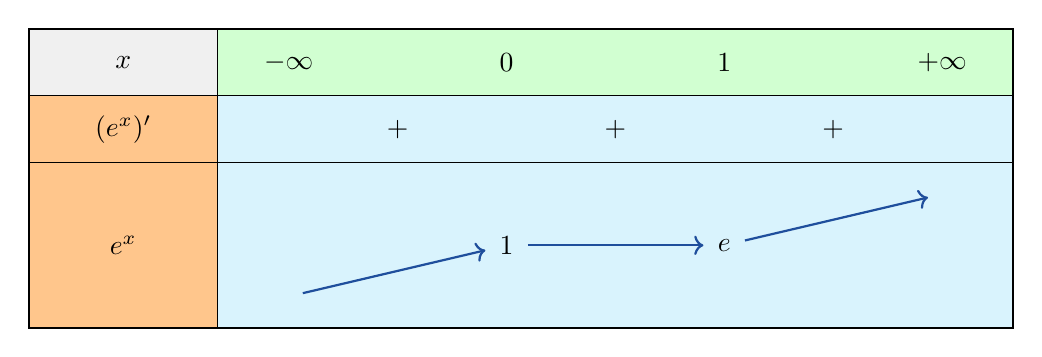
\begin{tikzpicture}[font=\normalsize]
\fill[gray!12] (0,0) rectangle (2.4,-0.85); \fill[green!18] (2.4,0) rectangle (12.5,-0.85);
\fill[orange!45] (0,-0.85) rectangle (2.4,-3.8); \fill[cyan!15] (2.4,-0.85) rectangle (12.5,-3.8);
\draw[thick] (0,0) rectangle (12.5,-3.8); \draw (0,-0.85)--(12.5,-0.85) (0,-1.7)--(12.5,-1.7) (2.4,0)--(2.4,-3.8);
\node at (1.2,-0.425){$x$}; \node at (1.2,-1.275){$(e^x)^{\prime}$}; \node at (1.2,-2.75){$e^x$};
\node at (3.3,-0.425){$-\infty$};
\node at (6.06667,-0.425){$0$};
\node at (8.83333,-0.425){$1$};
\node at (11.6,-0.425){$+\infty$};
\node at (4.68333,-1.275){$+$};
\node at (7.45,-1.275){$+$};
\node at (10.2167,-1.275){$+$};
\node[inner sep=2pt] (v0) at (3.3,-3.4){$$};
\node[inner sep=2pt] (v1) at (6.06667,-2.75){$1$};
\node[inner sep=2pt] (v2) at (8.83333,-2.75){$e$};
\node[inner sep=2pt] (v3) at (11.6,-2.1){$$};
\draw[->,cDef,thick,shorten <=3pt,shorten >=3pt] (v0)--(v1);
\draw[->,cDef,thick,shorten <=3pt,shorten >=3pt] (v1)--(v2);
\draw[->,cDef,thick,shorten <=3pt,shorten >=3pt] (v2)--(v3);
\end{tikzpicture}\end{LTR}\par \par\smallskip\begin{LTR}\centering 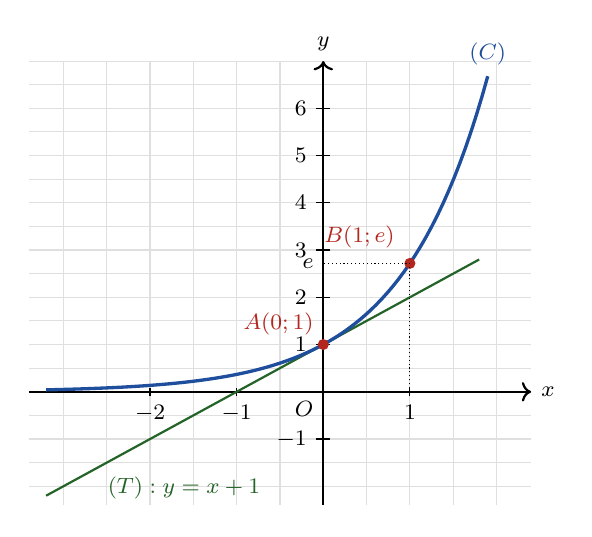
\begin{tikzpicture}[x=1.1cm,y=0.6cm,font=\footnotesize]\draw[gray!25,step=0.5] (-3.4,-2.4) grid (2.4,7);\draw[->,thick] (-3.4,0)--(2.4,0) node[right]{$x$}; \draw[->,thick] (0,-2.4)--(0,7) node[above]{$y$};\draw (-2,0.08)--(-2,-0.08) node[below]{$-2$};\draw (-1,0.08)--(-1,-0.08) node[below]{$-1$};\draw (1,0.08)--(1,-0.08) node[below]{$1$};\draw (0.08,-1)--(-0.08,-1) node[left]{$-1$};\draw (0.08,1)--(-0.08,1) node[left]{$1$};\draw (0.08,2)--(-0.08,2) node[left]{$2$};\draw (0.08,3)--(-0.08,3) node[left]{$3$};\draw (0.08,4)--(-0.08,4) node[left]{$4$};\draw (0.08,5)--(-0.08,5) node[left]{$5$};\draw (0.08,6)--(-0.08,6) node[left]{$6$};\node[below left] at (0,0){$O$};\draw[cRem!80!black,thick,domain=-3.2:1.8] plot (\x,{\x+1}); \node[cRem!80!black,below right] at (-2.6,-1.6){$(T):y=x+1$};
\draw[cDef,very thick,domain=-3.2:1.9,samples=80] plot (\x,{exp(\x)}) node[above]{$(C)$};
\fill[cThm] (0,1) circle (2pt) node[above left]{$A(0;1)$}; \fill[cThm] (1,2.718) circle (2pt) node[above left=2pt]{$B(1;e)$};
\draw[densely dotted] (1,0)--(1,2.718)--(0,2.718) node[left]{$e$};\end{tikzpicture}\end{LTR}\par }{}{}
\Row{}{%
\Lab{cMeth}{الوضع النسبي للمنحنى والمماس $(T)$}\ نضع $g(x)=e^x-(x+1)$:\par\textbf{(1)} $g^{\prime}(x)=e^x-1$: سالبة على $]-\infty;0[$ وموجبة على $]0;+\infty[$ ، إذن $g$ تبلغ قيمتها الحدية الصغرى $g(0)=0$.\par\textbf{(2)} إذن $g(x)\geqslant0$ ، أي $\RR{e^x\geqslant x+1}$:\par\smallskip\begin{LTR}\centering \begin{tikzpicture}[font=\normalsize]
\fill[gray!12] (0,0) rectangle (2.6,-0.9);
\fill[green!18] (2.6,0) rectangle (12.5,-0.9);
\fill[orange!45] (0,-0.9) rectangle (2.6,-4.6);
\fill[cyan!22] (2.6,-0.9) rectangle (12.5,-4.6);
\draw[thick] (0,0) rectangle (12.5,-4.6); \draw (0,-0.9)--(12.5,-0.9) (0,-1.8)--(12.5,-1.8) (2.6,0)--(2.6,-4.6);
\node at (1.3,-0.45){$x$};
\node at (1.3,-1.35){$e^x-(x+1)$};
\node[align=center,font=\bfseries] at (1.3,-3.2){\ar{الوضع}\\ \ar{النسبي}};
\node at (3.3,-0.45){$-\infty$};
\node at (7.55,-0.45){$0$};
\node at (11.8,-0.45){$+\infty$};
\node at (4.675,-1.35){$+$};
\node[align=center,font=\small] at (4.675,-3.2){$(C)$\\ \ar{فوق}\\ $(T)$};
\node at (10.425,-1.35){$+$};
\node[align=center,font=\small] at (10.425,-3.2){$(C)$\\ \ar{فوق}\\ $(T)$};
\node at (7.55,-1.35){$0$};
\draw[densely dotted] (7.55,-0.9)--(7.55,-1.13) (7.55,-1.57)--(7.55,-1.8);
\draw (6.05,-4.6) .. controls (6.125,-3.06) and (7.1,-2.136) .. (7.55,-1.8) .. controls (8,-2.136) and (8.975,-3.06) .. (9.05,-4.6);
\node[align=center,font=\footnotesize,inner sep=0pt] at (7.55,-3.65){\ar{$(C)$ يمس}\\ $(T)$\\ \ar{في النقطة}\\ $A(0;1)$};
\end{tikzpicture}\end{LTR}\par }{}{}
\Row{}{%
\Lab{cMeth}{حل معادلة أو متراجحة}\par\textbf{(1)} $\RR{e^{u(x)}=e^{v(x)}}$ تعني $\RR{u(x)=v(x)}$.\par\textbf{(2)} $\RR{e^{u(x)}\leqslant e^{v(x)}}$ تعني $\RR{u(x)\leqslant v(x)}$.}{}{}
\Row{}{%
\Lab{cEx}{أمثلة: حل في $\mathbb R$}\par\textbf{(1)} $e^x+2=0$: $e^x=-2$ مستحيلة لأن $e^x>0$: $\RR{S=\varnothing}$.\par\textbf{(2)} $e^{-2x+1}-1=0$: $e^{-2x+1}=e^0$ ، أي $-2x+1=0$: $\RR{S=\left\{\frac12\right\}}$.\par\textbf{(3)} $e^{x+1}=e^{\frac1x}$ مع $x\neq0$ ، تكافئ $x+1=\dfrac1x$ ، أي $x^2+x-1=0$.\par $\Delta=5$ ، والحلان غير معدومين: $\RR{S=\left\{\dfrac{-1-\sqrt5}2;\dfrac{-1+\sqrt5}2\right\}}$.\par\textbf{(4)} $e^{3x}\leqslant1$: $e^{3x}\leqslant e^0$ ، أي $3x\leqslant0$: $\RR{S=]-\infty;0]}$.\par\textbf{(5)} $e^{2x^2}\geqslant e^{5x+3}$ تكافئ $2x^2-5x-3\geqslant0$.\par $\Delta=49$ ، الجذران $-\dfrac12$ و $3$ ، والعبارة موجبة خارج الجذرين: $\RR{S=\left]-\infty;-\frac12\right]\cup[3;+\infty[}$.\par\textbf{(6)} $e^{2x}-(e+1)e^x+e=0$: نضع $X=e^x$ مع $X>0$ ، فنحصل على $X^2-(e+1)X+e=0$.\par $(X-1)(X-e)=0$ ، أي $X=1$ أو $X=e$ ، ومنه $e^x=e^0$ أو $e^x=e^1$: $\RR{S=\{0;1\}}$.}{}{}
\Row{}{%
\Lab{cThm!80!black}{حذار}\ في المتراجحة نحافظ على اتجاه التباين لأن الدالة الأسية متزايدة تمامًا.}{}{}
\Row{التقويم}{%
\Lab{cMeth}{تمرين تطبيقي}\par ادرس اتجاه تغير الدالة $f$ في كل حالة:\par\textbf{(1)} $f(x)=x+1+e^x$ ، $D_f=\mathbb R$.\par\textbf{(2)} $f(x)=\dfrac{e^x+1}{e^x-1}$ ، $D_f=]-\infty;0[\cup]0;+\infty[$.\par\textbf{(3)} $f(x)=(2x-3)e^x$ ، $D_f=\mathbb R$.}{25 د}{تقويم فردي.}
\Row{}{%
\Lab{cEx}{حل التمرين التطبيقي}\par\textbf{(1)} $f^{\prime}(x)=1+e^x>0$ ، إذن \RR{$f$} \RR{متزايدة} \RR{تمامًا} \RR{على} \RR{$\mathbb R$}.\par\textbf{(2)} $f^{\prime}(x)=\dfrac{e^x\big(e^x-1\big)-\big(e^x+1\big)e^x}{\big(e^x-1\big)^2}=\dfrac{-2e^x}{\big(e^x-1\big)^2}<0$ ، إذن \RR{$f$} \RR{متناقصة} \RR{تمامًا} \RR{على} \RR{كل} \RR{من} \RR{$]-\infty;0[$} \RR{و} \RR{$]0;+\infty[$}.\par\textbf{(3)} $f^{\prime}(x)=2e^x+(2x-3)e^x=\RR{(2x-1)e^x}$ ، وإشارتها إشارة $2x-1$ لأن $e^x>0$:\par\smallskip\begin{LTR}\centering 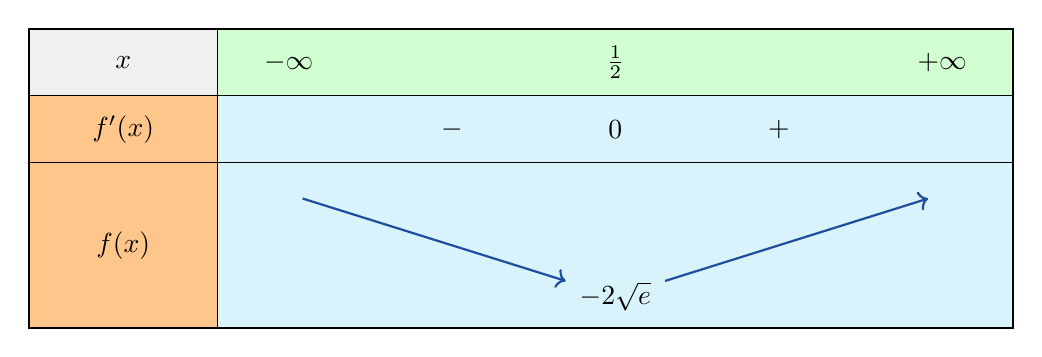
\begin{tikzpicture}[font=\normalsize]
\fill[gray!12] (0,0) rectangle (2.4,-0.85); \fill[green!18] (2.4,0) rectangle (12.5,-0.85);
\fill[orange!45] (0,-0.85) rectangle (2.4,-3.8); \fill[cyan!15] (2.4,-0.85) rectangle (12.5,-3.8);
\draw[thick] (0,0) rectangle (12.5,-3.8); \draw (0,-0.85)--(12.5,-0.85) (0,-1.7)--(12.5,-1.7) (2.4,0)--(2.4,-3.8);
\node at (1.2,-0.425){$x$}; \node at (1.2,-1.275){$f^{\prime}(x)$}; \node at (1.2,-2.75){$f(x)$};
\node at (3.3,-0.425){$-\infty$};
\node at (7.45,-0.425){$\frac12$};
\node at (11.6,-0.425){$+\infty$};
\node at (5.375,-1.275){$-$};
\node at (7.45,-1.275){$0$};
\node at (9.525,-1.275){$+$};
\node[inner sep=2pt] (v0) at (3.3,-2.1){$$};
\node[inner sep=2pt] (v1) at (7.45,-3.4){$-2\sqrt e$};
\node[inner sep=2pt] (v2) at (11.6,-2.1){$$};
\draw[->,cDef,thick,shorten <=3pt,shorten >=3pt] (v0)--(v1);
\draw[->,cDef,thick,shorten <=3pt,shorten >=3pt] (v1)--(v2);
\end{tikzpicture}\end{LTR}\par $f\left(\frac12\right)=(1-3)e^{\frac12}=\RR{-2\sqrt e}\approx-3{,}30$.\par\textbf{واجب منزلي:} التمارين 05 و 07 و 09 صفحة 102 ، ومن 29 إلى 36 صفحة 103.\par\smallskip\textbf{ملاحظات حول سير الحصة:} \dotfill}{}{}
\end{Sayr}
\newpage
\ModhHead{12}{3 ع ت}{تحليل}{الدالة الأسية}{02 سا}{دراسة الدوال $x\mapsto e^{u(x)}$ والدوال $x\mapsto e^{kx}$}%
{\begin{itemize}\item اتجاه تغير مركب دالتين ، مشتقة دالة مركبة.\end{itemize}}%
{\begin{itemize}\item تعيين اتجاه تغير ومشتقة الدالة $x\mapsto e^{u(x)}$.\item توظيف الدوال $x\mapsto e^{kx}$ في النمذجة.\end{itemize}}%
{المنهاج ، الكتاب المدرسي ، الآلة الحاسبة العلمية ، برمجية Geogebra.}
\begin{Sayr}
\Row{مرحلة الانطلاق}{%
\textbf{التهيئة النفسية:} التذكير بمشتقة دالة مركبة: $(g\circ u)^{\prime}=u^{\prime}\times g^{\prime}\circ u$.}{10 د}{تذكير بمشتقة مركب.}
\Row{التشخيص والاكتشاف}{%
\Lab{cEx}{نشاط رقم 03}\ $f(x)=e^{2x+7}$ على $\mathbb R$.\par\textbf{(1)} اكتب $f$ على شكل مركب دالتين.\par\textbf{(2)} استنتج اتجاه تغير $f$.\par\textbf{(3)} احسب $f^{\prime}(x)$.}{35 د}{مناقشة النشاط.}
\Row{}{%
\Lab{cDef}{مناقشة النشاط}\par\textbf{(1)} $f=\exp\circ u$ حيث $u(x)=2x+7$.\par\textbf{(2)} $u$ و $\exp$ متزايدتان تمامًا ، إذن \RR{$f$} \RR{متزايدة} \RR{تمامًا} \RR{على} \RR{$\mathbb R$}.\par\textbf{(3)} $f^{\prime}(x)=u^{\prime}(x)\times e^{u(x)}=\RR{2e^{2x+7}}$.}{}{}
\Row{بناء المعارف}{%
\Lab{cThm}{اتجاه التغير}\ إذا كانت $u$ معرفة على مجال $I$ فإن للدالتين $u$ و $\exp\circ u$ \RR{نفس} \RR{اتجاه} \RR{التغير} على $I$.}{50 د}{مثال نمذجة من الواقع.}
\Row{}{%
\Lab{cMeth}{البرهان}\ الدالة $\exp$ متزايدة تمامًا على $\mathbb R$ ، وحسب مبرهنة اتجاه تغير مركب دالتين: إذا كان لـ $u$ و $\exp$ نفس الاتجاه فإن $\exp\circ u$ متزايدة ، وإلا فهي متناقصة.}{}{}
\Row{}{%
\Lab{cThm}{المشتقة}\ إذا كانت $u$ قابلة للاشتقاق على $I$ فإن: $\RR{\big[e^{u(x)}\big]^{\prime}=u^{\prime}(x)\,e^{u(x)}}$.}{}{}
\Row{}{%
\Lab{cEx}{أمثلة}\par\textbf{(1)} $f(x)=e^{x^2-3x+1}$: $\RR{f^{\prime}(x)=(2x-3)e^{x^2-3x+1}}$.\par\textbf{(2)} $g(x)=e^{\sqrt x}$ على $]0;+\infty[$: $\RR{g^{\prime}(x)=\dfrac1{2\sqrt x}e^{\sqrt x}}$.}{}{}
\Row{}{%
\Lab{cThm}{حالة خاصة: الدوال $x\mapsto e^{kx}$}\par\textbf{(1)} $\big(e^{kx}\big)^{\prime}=ke^{kx}$.\par\textbf{(2)} إذا كان $k>0$: $x\mapsto e^{kx}$ \RR{متزايدة} \RR{تمامًا} (نمو).\par\textbf{(3)} إذا كان $k<0$: $x\mapsto e^{kx}$ \RR{متناقصة} \RR{تمامًا} (تناقص).}{}{}
\Row{}{%
\Lab{cEx}{نمذجة}\ عدد سكان مدينة (بالآلاف) بعد $t$ سنة: $P(t)=1000\,e^{0{,}02t}$.\par\textbf{(1)} $k=0{,}02>0$: \RR{$P$} \RR{متزايدة} (السكان يتزايدون).\par\textbf{(2)} $P(0)=\RR{1000}$ ألف ، و $P(10)=1000e^{0{,}2}\approx\RR{1221{,}4}$ ألف.}{}{}
\Row{}{%
\Lab{cThm!80!black}{حذار}\ $\big(e^{u}\big)^{\prime}=u^{\prime}e^{u}$ وليست $e^{u^{\prime}}$.}{}{}
\Row{التقويم}{%
\Lab{cMeth}{تمرين تطبيقي}\par ادرس اتجاه تغير الدالة $f$ في كل حالة:\par\textbf{(1)} $f(x)=x+1-e^{-2x}$ ، $D_f=\mathbb R$.\par\textbf{(2)} $f(x)=e^{3x}-3e^x$ ، $D_f=\mathbb R$.\par\textbf{(3)} $f(x)=\dfrac{e^{4x}-3}{e^{4x}+1}$ ، $D_f=\mathbb R$.\par\textbf{(4)} $f(x)=e^{\frac{x+1}{x-1}}$ ، $D_f=]-\infty;1[\cup]1;+\infty[$.}{25 د}{تقويم فردي.}
\Row{}{%
\Lab{cEx}{حل التمرين التطبيقي}\par\textbf{(1)} $f^{\prime}(x)=1-(-2)e^{-2x}=1+2e^{-2x}>0$: \RR{$f$} \RR{متزايدة} \RR{تمامًا} \RR{على} \RR{$\mathbb R$}.\par\textbf{(2)} $f^{\prime}(x)=3e^{3x}-3e^x=3e^x\big(e^{2x}-1\big)$ ، وإشارتها إشارة $e^{2x}-1$: موجبة إذا كان $2x>0$:\par\smallskip\begin{LTR}\centering 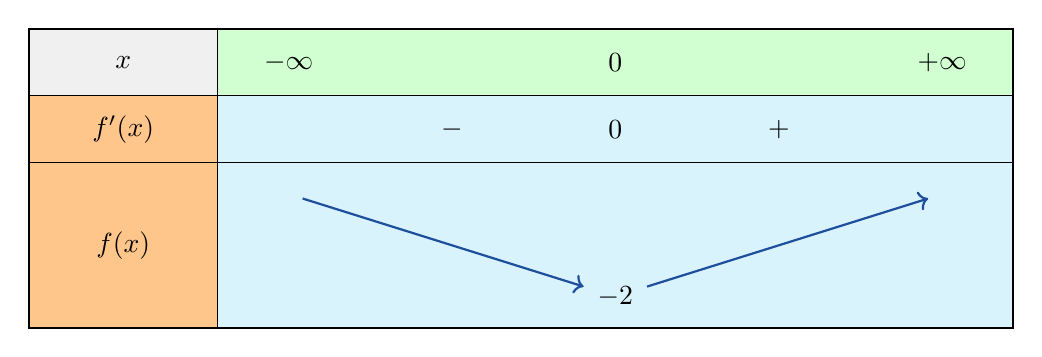
\begin{tikzpicture}[font=\normalsize]
\fill[gray!12] (0,0) rectangle (2.4,-0.85); \fill[green!18] (2.4,0) rectangle (12.5,-0.85);
\fill[orange!45] (0,-0.85) rectangle (2.4,-3.8); \fill[cyan!15] (2.4,-0.85) rectangle (12.5,-3.8);
\draw[thick] (0,0) rectangle (12.5,-3.8); \draw (0,-0.85)--(12.5,-0.85) (0,-1.7)--(12.5,-1.7) (2.4,0)--(2.4,-3.8);
\node at (1.2,-0.425){$x$}; \node at (1.2,-1.275){$f^{\prime}(x)$}; \node at (1.2,-2.75){$f(x)$};
\node at (3.3,-0.425){$-\infty$};
\node at (7.45,-0.425){$0$};
\node at (11.6,-0.425){$+\infty$};
\node at (5.375,-1.275){$-$};
\node at (7.45,-1.275){$0$};
\node at (9.525,-1.275){$+$};
\node[inner sep=2pt] (v0) at (3.3,-2.1){$$};
\node[inner sep=2pt] (v1) at (7.45,-3.4){$-2$};
\node[inner sep=2pt] (v2) at (11.6,-2.1){$$};
\draw[->,cDef,thick,shorten <=3pt,shorten >=3pt] (v0)--(v1);
\draw[->,cDef,thick,shorten <=3pt,shorten >=3pt] (v1)--(v2);
\end{tikzpicture}\end{LTR}\par $f(0)=1-3=\RR{-2}$.\par\textbf{(3)} $f^{\prime}(x)=\dfrac{4e^{4x}\big(e^{4x}+1\big)-4e^{4x}\big(e^{4x}-3\big)}{\big(e^{4x}+1\big)^2}=\dfrac{16e^{4x}}{\big(e^{4x}+1\big)^2}>0$: \RR{$f$} \RR{متزايدة} \RR{تمامًا} \RR{على} \RR{$\mathbb R$}.\par\textbf{(4)} $u(x)=\dfrac{x+1}{x-1}$ ، $u^{\prime}(x)=\dfrac{(x-1)-(x+1)}{(x-1)^2}=\dfrac{-2}{(x-1)^2}<0$:\par $f^{\prime}(x)=\dfrac{-2}{(x-1)^2}e^{\frac{x+1}{x-1}}<0$: \RR{$f$} \RR{متناقصة} \RR{تمامًا} \RR{على} \RR{كل} \RR{من} \RR{المجالين}.\par\textbf{واجب منزلي:} التمرينان 38 و 39 صفحة 104.\par\smallskip\textbf{ملاحظات حول سير الحصة:} \dotfill}{}{}
\end{Sayr}
\newpage
\ModhHead{13}{3 ع ت}{تحليل}{الدالة الأسية}{02 سا}{المعادلات التفاضلية $y^{\prime}=ay$ و $y^{\prime}=ay+b$}%
{\begin{itemize}\item الدالة الأسية ، مشتقة $x\mapsto e^{kx}$ ، المعادلات التفاضلية $y^{\prime}=f$.\end{itemize}}%
{\begin{itemize}\item حل معادلة تفاضلية من الشكل $y^{\prime}=ay+b$.\item تعيين الحل الذي يحقق شرطًا ابتدائيًا.\end{itemize}}%
{المنهاج ، الكتاب المدرسي ، الآلة الحاسبة العلمية ، برمجية Geogebra.}
\begin{Sayr}
\Row{مرحلة الانطلاق}{%
\textbf{التهيئة النفسية:} المعادلة التفاضلية معادلة مجهولها دالة $y$ وتربط بين $y$ ومشتقتها $y^{\prime}$.}{10 د}{تعريف المعادلة التفاضلية.}
\Row{التشخيص والاكتشاف}{%
\Lab{cEx}{نشاط رقم 04}\ $a$ و $c$ عددان حقيقيان ، $a\neq0$.\par\textbf{(1)} $f(x)=ce^{ax}$: احسب $f^{\prime}(x)$ وتحقق أن $f^{\prime}=af$.\par\textbf{(2)} تحقق أن الدالة الثابتة $x\mapsto-\dfrac ba$ حل للمعادلة $y^{\prime}=ay+b$.}{35 د}{التحقق بالاشتقاق.}
\Row{}{%
\Lab{cDef}{مناقشة النشاط}\par\textbf{(1)} $f^{\prime}(x)=c\times ae^{ax}=a\big(ce^{ax}\big)=\RR{af(x)}$: $f$ حل للمعادلة $y^{\prime}=ay$.\par\textbf{(2)} مشتقة الثابت معدومة ، و $a\left(-\dfrac ba\right)+b=-b+b=\RR{0}$: الدالة الثابتة حل.}{}{}
\Row{بناء المعارف}{%
\Lab{cThm}{مبرهنة 1}\ $a$ عدد حقيقي غير معدوم. حلول المعادلة $y^{\prime}=ay$ على $\mathbb R$ هي الدوال $\RR{x\mapsto ce^{ax}}$ حيث $c$ عدد حقيقي ثابت.}{50 د}{البرهان مع التلاميذ.}
\Row{}{%
\Lab{cMeth}{البرهان}\ لتكن $g$ حلًا ، نضع $h(x)=g(x)e^{-ax}$: $h^{\prime}(x)=g^{\prime}(x)e^{-ax}-ag(x)e^{-ax}=\big(ag(x)-ag(x)\big)e^{-ax}=0$.\par إذن $h$ ثابتة: $h(x)=c$ ، ومنه $g(x)=ce^{ax}$.}{}{}
\Row{}{%
\Lab{cThm}{مبرهنة 2}\ $a\neq0$. حلول المعادلة $y^{\prime}=ay+b$ على $\mathbb R$ هي الدوال $\RR{x\mapsto ce^{ax}-\dfrac ba}$ حيث $c$ ثابت حقيقي.}{}{}
\Row{}{%
\Lab{cThm}{الحل الذي يحقق شرطًا}\ من أجل كل ثنائية $(x_0;y_0)$ ، المعادلة $y^{\prime}=ay+b$ ($a\neq0$) تقبل \RR{حلًا} \RR{وحيدًا} $f$ يحقق $f(x_0)=y_0$.}{}{}
\Row{}{%
\Lab{cEx}{أمثلة}\par\textbf{(1)} $y^{\prime}+5y=0$ معناه $y^{\prime}=-5y$: الحلول $\RR{x\mapsto ce^{-5x}}$ ، $c\in\mathbb R$.\par\textbf{(2)} $y^{\prime}=2y+1$: $a=2$ ، $b=1$: الحلول $\RR{x\mapsto ce^{2x}-\dfrac12}$.\par\textbf{(3)} الحل الذي يحقق $f(0)=1$: $c-\dfrac12=1$ ، $c=\dfrac32$: $\RR{f(x)=\dfrac32e^{2x}-\dfrac12}$.}{}{}
\Row{}{%
\Lab{cThm!80!black}{حذار}\ نكتب المعادلة على الشكل $y^{\prime}=ay+b$ قبل تطبيق المبرهنة.}{}{}
\Row{التقويم}{%
\Lab{cMeth}{تمرين تطبيقي}\par نعتبر المعادلة التفاضلية $(E):\ 2y^{\prime}+y=1$.\par\textbf{(1)} حل في $\mathbb R$ المعادلة $(E)$.\par\textbf{(2)} عيّن الحل الخاص $f$ للمعادلة $(E)$ بحيث $f(-1)=2$.\par\textbf{(3)} ادرس اتجاه تغير $f$ ، والوضع النسبي لمنحناها والمستقيم $y=1$ ، ثم ارسم $(C_f)$.}{25 د}{نهاية محور الدالة الأسية.}
\Row{}{%
\Lab{cEx}{حل التمرين التطبيقي}\par\textbf{(1)} $(E)$ تكافئ $y^{\prime}=-\dfrac12y+\dfrac12$: $a=-\dfrac12$ ، $b=\dfrac12$ ، $-\dfrac ba=1$:\par الحلول $\RR{x\mapsto ce^{-\frac x2}+1}$ ، $c\in\mathbb R$.\par\textbf{(2)} $f(-1)=ce^{\frac12}+1=2$ ، $c=e^{-\frac12}$: $\RR{f(x)=e^{-\frac{x+1}2}+1}$.\par\textbf{(3)} $f^{\prime}(x)=-\dfrac12e^{-\frac{x+1}2}<0$: \RR{$f$} \RR{متناقصة} \RR{تمامًا} \RR{على} \RR{$\mathbb R$}.\par $f(x)-1=e^{-\frac{x+1}2}>0$: \RR{$(C_f)$} \RR{فوق} \RR{المستقيم} \RR{$(\Delta):y=1$}.\par\smallskip\begin{LTR}\centering \begin{tikzpicture}[font=\normalsize]
\fill[gray!12] (0,0) rectangle (2.6,-0.9);
\fill[green!18] (2.6,0) rectangle (12.5,-0.9);
\fill[orange!45] (0,-0.9) rectangle (2.6,-4.6);
\fill[cyan!22] (2.6,-0.9) rectangle (12.5,-4.6);
\draw[thick] (0,0) rectangle (12.5,-4.6); \draw (0,-0.9)--(12.5,-0.9) (0,-1.8)--(12.5,-1.8) (2.6,0)--(2.6,-4.6);
\node at (1.3,-0.45){$x$};
\node at (1.3,-1.35){$f(x)-1$};
\node[align=center,font=\bfseries] at (1.3,-3.2){\ar{الوضع}\\ \ar{النسبي}};
\node at (3.3,-0.45){$-\infty$};
\node at (11.8,-0.45){$+\infty$};
\node at (7.55,-1.35){$+$};
\node[align=center,font=\small] at (7.55,-3.2){$(C_f)$\\ \ar{فوق}\\ $(\Delta)$};
\end{tikzpicture}\end{LTR}\par \par\smallskip\begin{LTR}\centering 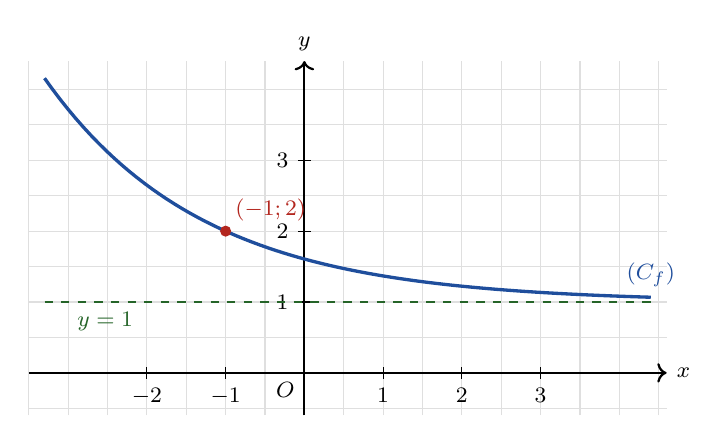
\begin{tikzpicture}[x=1cm,y=0.9cm,font=\footnotesize]\draw[gray!25,step=0.5] (-3.5,-0.6) grid (4.6,4.4);\draw[->,thick] (-3.5,0)--(4.6,0) node[right]{$x$}; \draw[->,thick] (0,-0.6)--(0,4.4) node[above]{$y$};\draw (-2,0.08)--(-2,-0.08) node[below]{$-2$};\draw (-1,0.08)--(-1,-0.08) node[below]{$-1$};\draw (1,0.08)--(1,-0.08) node[below]{$1$};\draw (2,0.08)--(2,-0.08) node[below]{$2$};\draw (3,0.08)--(3,-0.08) node[below]{$3$};\draw (0.08,1)--(-0.08,1) node[left]{$1$};\draw (0.08,2)--(-0.08,2) node[left]{$2$};\draw (0.08,3)--(-0.08,3) node[left]{$3$};\node[below left] at (0,0){$O$};\draw[cRem!80!black,thick,dashed] (-3.3,1)--(4.4,1) node[pos=0.1,below]{$y=1$};
\draw[cDef,very thick,domain=-3.3:4.4,samples=80] plot (\x,{exp(-(\x+1)/2)+1}) node[above]{$(C_f)$};
\fill[cThm] (-1,2) circle (2pt) node[above right]{$(-1;2)$};\end{tikzpicture}\end{LTR}\par \par\textbf{واجب منزلي:} التمرين 102 صفحة 109 ، والتمرينان 105 و 106 صفحة 110.\par\smallskip\textbf{ملاحظات حول سير الحصة:} \dotfill}{}{}
\end{Sayr}
\end{document}
